% Options for packages loaded elsewhere
\PassOptionsToPackage{unicode}{hyperref}
\PassOptionsToPackage{hyphens}{url}
%
\documentclass[
  12pt,
]{article}
\usepackage{lmodern}
\usepackage{amsmath}
\usepackage{ifxetex,ifluatex}
\ifnum 0\ifxetex 1\fi\ifluatex 1\fi=0 % if pdftex
  \usepackage[T1]{fontenc}
  \usepackage[utf8]{inputenc}
  \usepackage{textcomp} % provide euro and other symbols
  \usepackage{amssymb}
\else % if luatex or xetex
  \usepackage{unicode-math}
  \defaultfontfeatures{Scale=MatchLowercase}
  \defaultfontfeatures[\rmfamily]{Ligatures=TeX,Scale=1}
  \setmainfont[]{Times New Roman}
\fi
% Use upquote if available, for straight quotes in verbatim environments
\IfFileExists{upquote.sty}{\usepackage{upquote}}{}
\IfFileExists{microtype.sty}{% use microtype if available
  \usepackage[]{microtype}
  \UseMicrotypeSet[protrusion]{basicmath} % disable protrusion for tt fonts
}{}
\makeatletter
\@ifundefined{KOMAClassName}{% if non-KOMA class
  \IfFileExists{parskip.sty}{%
    \usepackage{parskip}
  }{% else
    \setlength{\parindent}{0pt}
    \setlength{\parskip}{6pt plus 2pt minus 1pt}}
}{% if KOMA class
  \KOMAoptions{parskip=half}}
\makeatother
\usepackage{xcolor}
\IfFileExists{xurl.sty}{\usepackage{xurl}}{} % add URL line breaks if available
\IfFileExists{bookmark.sty}{\usepackage{bookmark}}{\usepackage{hyperref}}
\hypersetup{
  pdftitle={Feelings about fish: An analysis of social survey results about seafood},
  pdfauthor={Zoe Wong, Molly Bruce},
  hidelinks,
  pdfcreator={LaTeX via pandoc}}
\urlstyle{same} % disable monospaced font for URLs
\usepackage[margin=2.54cm]{geometry}
\usepackage{longtable,booktabs}
\usepackage{calc} % for calculating minipage widths
% Correct order of tables after \paragraph or \subparagraph
\usepackage{etoolbox}
\makeatletter
\patchcmd\longtable{\par}{\if@noskipsec\mbox{}\fi\par}{}{}
\makeatother
% Allow footnotes in longtable head/foot
\IfFileExists{footnotehyper.sty}{\usepackage{footnotehyper}}{\usepackage{footnote}}
\makesavenoteenv{longtable}
\usepackage{graphicx}
\makeatletter
\def\maxwidth{\ifdim\Gin@nat@width>\linewidth\linewidth\else\Gin@nat@width\fi}
\def\maxheight{\ifdim\Gin@nat@height>\textheight\textheight\else\Gin@nat@height\fi}
\makeatother
% Scale images if necessary, so that they will not overflow the page
% margins by default, and it is still possible to overwrite the defaults
% using explicit options in \includegraphics[width, height, ...]{}
\setkeys{Gin}{width=\maxwidth,height=\maxheight,keepaspectratio}
% Set default figure placement to htbp
\makeatletter
\def\fps@figure{htbp}
\makeatother
\setlength{\emergencystretch}{3em} % prevent overfull lines
\providecommand{\tightlist}{%
  \setlength{\itemsep}{0pt}\setlength{\parskip}{0pt}}
\setcounter{secnumdepth}{5}
\ifluatex
  \usepackage{selnolig}  % disable illegal ligatures
\fi

\title{Feelings about fish: An analysis of social survey results about
seafood}
\usepackage{etoolbox}
\makeatletter
\providecommand{\subtitle}[1]{% add subtitle to \maketitle
  \apptocmd{\@title}{\par {\large #1 \par}}{}{}
}
\makeatother
\subtitle{\url{https://github.com/ztw814/ENV872_FinalProject}}
\author{Zoe Wong, Molly Bruce}
\date{}

\begin{document}
\maketitle

\newpage
\tableofcontents 
\newpage
\listoffigures 
\newpage

\hypertarget{rationale-and-research-questions}{%
\section{Rationale and Research
Questions}\label{rationale-and-research-questions}}

According to catch reconstructions, global fishing rates peaked in 1996
at roughly 130 million tons of fished biomass or, according to reported
catches, at roughly 85 million tons that same year (Pauly \& Zeller
2016). In the wake of this peak and an accompanying recognition that
seafood extraction remains unsustainable, many researchers have become
increasingly interested in understanding how communities interact with
seafood consumption, seafood sustainability, etc. Understanding how
consumers and communities interact with seafood and sustainability
concepts is the first, crucial step in beginning to to make more
comprehensive progress toward achieving sustainable seafood extraction.
This background sets the stage for both this data examination as well as
the original research that collected the data on which this examination
relies.

\hypertarget{research-questions}{%
\subsection{Research Questions}\label{research-questions}}

\begin{enumerate}
\def\labelenumi{\arabic{enumi}.}
\item
  \begin{enumerate}
  \def\labelenumii{(\alph{enumii})}
  \tightlist
  \item
    When consumers buy seafood, which species do they prefer? (b) Do
    they prefer wild or farmed fish?
  \end{enumerate}
\item
  \begin{enumerate}
  \def\labelenumii{(\alph{enumii})}
  \tightlist
  \item
    What qualities do consumers associate with wild vs.~farmed seafood?
    (b) What qualities do they value in seafood?
  \end{enumerate}
\item
  Are seafood values predicted by demographic variables such as age or
  education level?
\end{enumerate}

\newpage

\hypertarget{dataset-information}{%
\section{Dataset Information}\label{dataset-information}}

\hypertarget{description-of-the-data}{%
\subsection{Description of the Data}\label{description-of-the-data}}

Our data were obtained from a social science survey conducted by a
multi-university team of researchers, including the Murray lab at Duke
University. The survey was conducted in the summer of 2020 via Qualtrics
and targeted North Carolina residents from across the state.

The survey asked respondents a total of 37 questions. The question
topics can be broken down into the following categories: eating habits
for 8 types of seafood, what qualities respondents associate with
seafood, attitudes about mariculture, attitudes about North Carolina
seafood versus commercial fishing, respondents' involvement with seafood
production, and demographic indicators. This study focuses on questions
about eating habits, what qualities are associated with seafood, and
demographic indicators.

Respondents answered each question by selecting one option from a menu
of choices; the number of choices available depended on the question.
The dataset contained responses from 1436 participants.

\hypertarget{data-wrangling}{%
\subsection{Data Wrangling}\label{data-wrangling}}

For each analysis, we created a new dataset containing only the relevant
columns. For each category within the survey question, we then created a
table with the frequency of each questions response. For example, one
question asked respondents to rate how often they ate each of 8 types of
seafood; respondents could choose from 7 responses for each seafood
type. To wrangle this data, we created a dataframe for each type of
seafood, for a total of 8 dataframes, each of which contained a column
with the response choices and a column with the number of respondents
that chose each response. Because the response choices were only
represented by a number in the raw data, we renamed the response column
with the meaning of each number for greater clarity. We repeated this
process for the first two research questions (how often participants eat
each type of seafood, whether participants prefer each type wild or
farmed, whether participants associate each quality with wild or farmed
seafood).

For the third research question, we created a dataframe with responses
to a question about how important each of 11 qualities was when
respondents were buying seafood. We then renamed the columns and removed
rows with alternate responses to demographic variables, such as ``prefer
not to answer.''

\hypertarget{data-structure-consumer-preferences}{%
\subsection{Data Structure: Consumer
preferences}\label{data-structure-consumer-preferences}}

****Data from these responses are categorical, but the response choices
could be situated along a linear scale, allowing us to analyze response
means.

\begin{longtable}[]{@{}lll@{}}
\toprule
\begin{minipage}[b]{(\columnwidth - 2\tabcolsep) * \real{0.34}}\raggedright
Research Question\strut
\end{minipage} &
\begin{minipage}[b]{(\columnwidth - 2\tabcolsep) * \real{0.41}}\raggedright
Survey Question\strut
\end{minipage} &
\begin{minipage}[b]{(\columnwidth - 2\tabcolsep) * \real{0.25}}\raggedright
Response choices\strut
\end{minipage}\tabularnewline
\midrule
\endhead
\begin{minipage}[t]{(\columnwidth - 2\tabcolsep) * \real{0.34}}\raggedright
1a. When consumers buy seafood, which species do they prefer?\strut
\end{minipage} &
\begin{minipage}[t]{(\columnwidth - 2\tabcolsep) * \real{0.41}}\raggedright
In the past year, how often did you eat the following type of
seafood**?\strut
\end{minipage} &
\begin{minipage}[t]{(\columnwidth - 2\tabcolsep) * \real{0.25}}\raggedright
0 = Never, 1 = Once in the past year, 2 = A few times in the past year,
3 = Once a month, 4 = A few times every month, 5 = Once a week, 6 = More
than once a week\strut
\end{minipage}\tabularnewline
\begin{minipage}[t]{(\columnwidth - 2\tabcolsep) * \real{0.34}}\raggedright
1b. Do consumers prefer wild or farmed fish?\strut
\end{minipage} &
\begin{minipage}[t]{(\columnwidth - 2\tabcolsep) * \real{0.41}}\raggedright
Between wild-caught and farmed versions of the same seafood species**,
which do you prefer to eat?\strut
\end{minipage} &
\begin{minipage}[t]{(\columnwidth - 2\tabcolsep) * \real{0.25}}\raggedright
1 = Strongly prefer wild-caught, 2 = Slightly prefer wild-caught, 3 = No
preference, 4 = Slightly prefer farmed, 5 = Strongly prefer farmed, 6 =
I don't know\strut
\end{minipage}\tabularnewline
\begin{minipage}[t]{(\columnwidth - 2\tabcolsep) * \real{0.34}}\raggedright
2a. What qualities do consumers associate with wild vs.~farmed
seafood?\strut
\end{minipage} &
\begin{minipage}[t]{(\columnwidth - 2\tabcolsep) * \real{0.41}}\raggedright
How do you associate the following qualities*** with different types of
seafood (farmed and wild-caught)?\strut
\end{minipage} &
\begin{minipage}[t]{(\columnwidth - 2\tabcolsep) * \real{0.25}}\raggedright
1 = More associated with wild-caught, 2 = Associated equally with
wild-caught and farmed, 3 = More associated with farmed, 4 = Associated
with neither wild-caught or farmed, 5 = I don't know\strut
\end{minipage}\tabularnewline
\begin{minipage}[t]{(\columnwidth - 2\tabcolsep) * \real{0.34}}\raggedright
2b. What qualities do consumers value in seafood?\strut
\end{minipage} &
\begin{minipage}[t]{(\columnwidth - 2\tabcolsep) * \real{0.41}}\raggedright
When you are buying seafood, how important are the following
qualities*** to you?\strut
\end{minipage} &
\begin{minipage}[t]{(\columnwidth - 2\tabcolsep) * \real{0.25}}\raggedright
1 = Not at all important, 2 = Slightly important, 3 = Moderately
important, 4 = Very important, 5 = Extremely important\strut
\end{minipage}\tabularnewline
\bottomrule
\end{longtable}

** Seafood types: Tuna, Shrimp, Salmon, Flounder, Blue Crab, Clams,
Mullet, Oysters (8)

*** Qualities: Healthy, Local, Safe, Tasty, Affordable, Sustainable,
Fresh, Easy Access, Local Culture, Local Economies, Local Environment
(11)

\hypertarget{data-structure-demographics}{%
\subsection{Data structure:
Demographics}\label{data-structure-demographics}}

\begin{longtable}[]{@{}lll@{}}
\toprule
Demographic Category & Response choices & Counts\tabularnewline
\midrule
\endhead
Age & 1=19 or younger & 74\tabularnewline
. & 2=20-29 & 201\tabularnewline
. & 3=30-39 & 170\tabularnewline
. & 4=40-49 & 159\tabularnewline
. & 5=50-59 & 156\tabularnewline
. & 6=60-69 & 172\tabularnewline
. & 7=70 or older & 100\tabularnewline
. & 8=Prefer not to answer & 8\tabularnewline
Education level & 1=Less than high school & 35\tabularnewline
. & 2=High school graduate & 229\tabularnewline
. & 3=Some college & 302\tabularnewline
. & 4=2 year degree & 167\tabularnewline
. & 5=4 year degree & 382\tabularnewline
. & 6=Professional degree & 260\tabularnewline
. & 7=Doctorate & 49\tabularnewline
. & 8=Prefer not to answer & 12\tabularnewline
Political party & 1=Republican & 449\tabularnewline
. & 2=Democrat & 459\tabularnewline
. & 3=Independent & 384\tabularnewline
. & 4=Other & 28\tabularnewline
. & 5=Prefer not to answer & 116\tabularnewline
\bottomrule
\end{longtable}

\newpage

\hypertarget{exploratory-analysis}{%
\section{Exploratory Analysis}\label{exploratory-analysis}}

Below, we explore and visualize how often respondents consume select
seafood products, regardless of the seafood species.

\begin{figure}
\centering
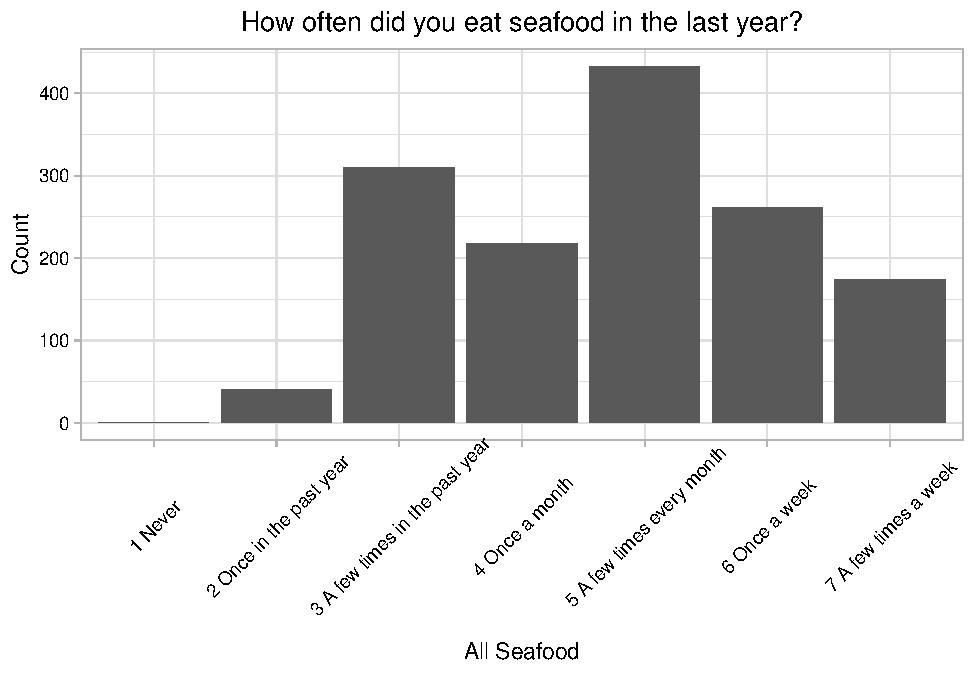
\includegraphics{Final_rmd_files/figure-latex/freq general-1.pdf}
\caption{Bar plot of the frequency of general seafood consumption}
\end{figure}

Figure 1 shows the distribution of responses regarding frequency of
seafood consumption in the last year. The mean frequency reported for
all seafood consumption was 4.76. This means that the average respondent
ate seafood between once a month and a few times per month.

\newpage

\hypertarget{analysis}{%
\section{Analysis}\label{analysis}}

\hypertarget{question-1a-when-consumers-buy-seafood-which-species-do-they-prefer}{%
\subsection{Question 1a: When consumers buy seafood, which species do
they
prefer?}\label{question-1a-when-consumers-buy-seafood-which-species-do-they-prefer}}

Figure 2 shows that respondents tend to eat Shrimp, Tuna, and Salmon
more often than they eat the other species. Respondents overwhelmingly
never eat Mullet. Respondents seem to eat Blue Crab, Clams, and Oysters
very infrequently if ever. However, this information is still pulled
apart by frequency. The below visualization simplifies the data even
further, capturing the number of respondents who ever consume each
species.

\begin{figure}
\centering
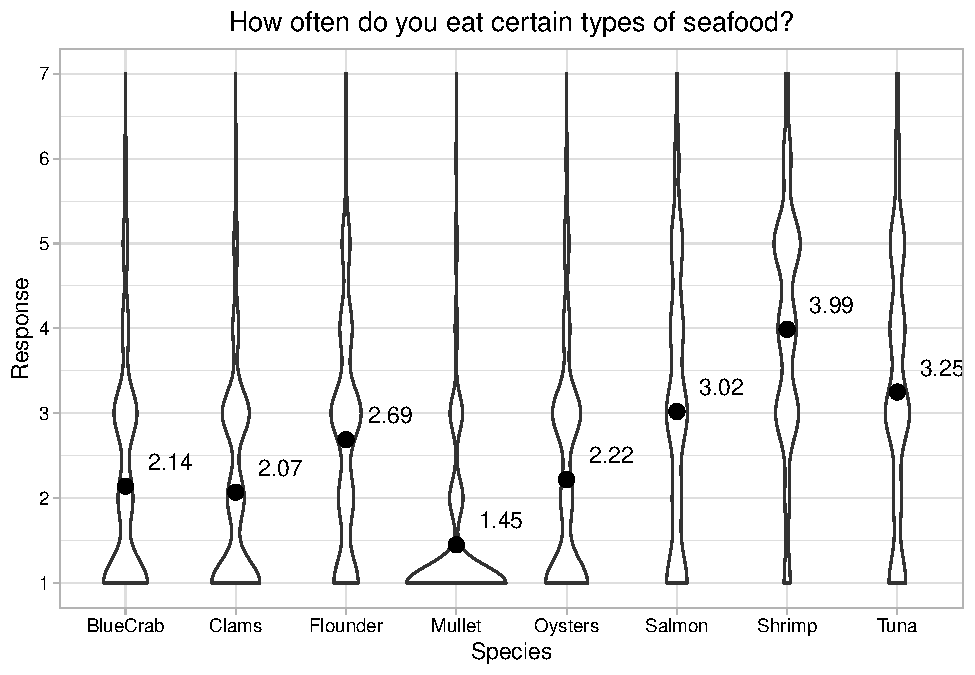
\includegraphics{Final_rmd_files/figure-latex/freq violin-1.pdf}
\caption{Violin plot and means of the frequency of seafood consumption
based on type}
\end{figure}

\begin{figure}
\centering
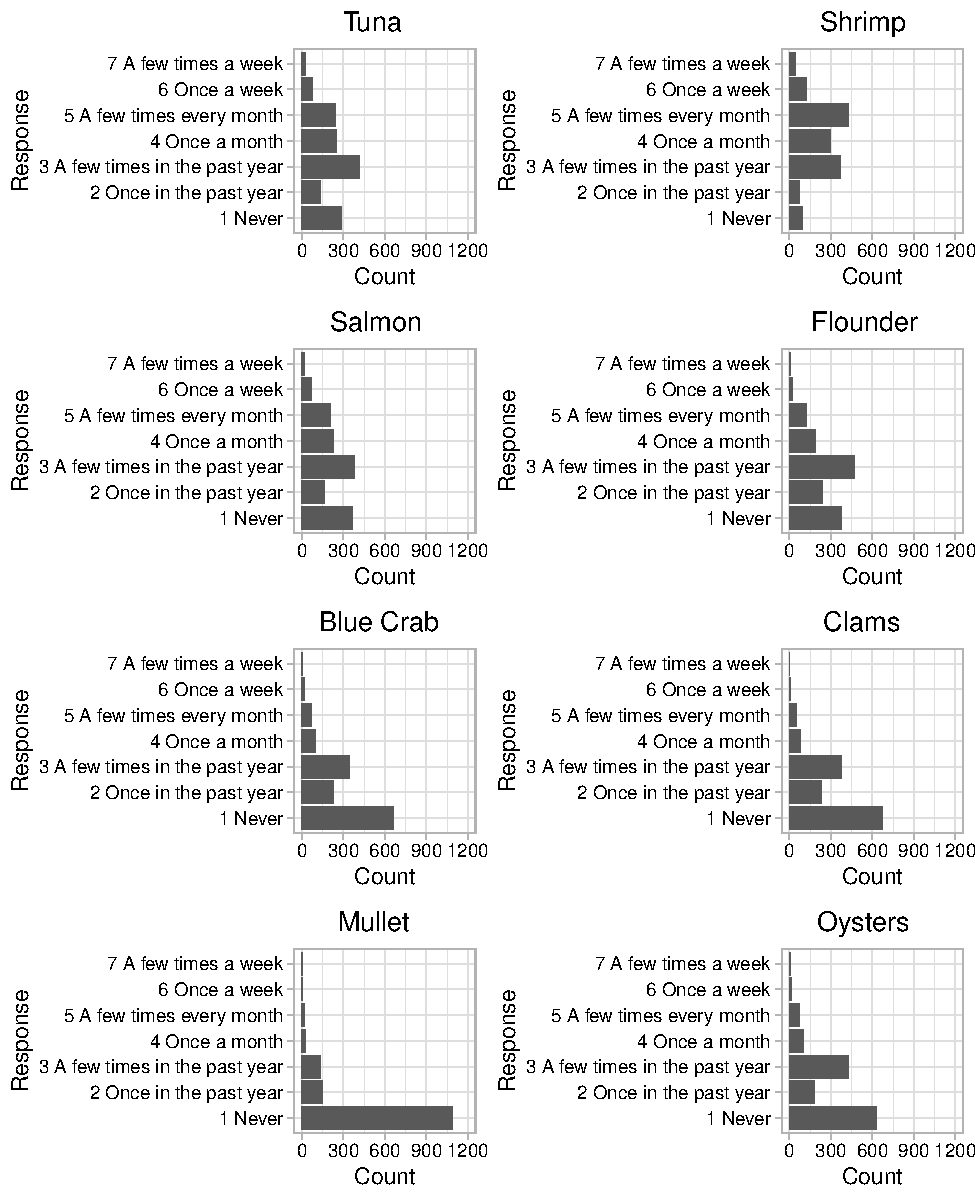
\includegraphics{Final_rmd_files/figure-latex/frequency-1.pdf}
\caption{Bar plot of the frequency of seafood consumption based on type}
\end{figure}

\hypertarget{question-1b-do-consumers-prefer-wild-or-farmed-fish}{%
\subsubsection{Question 1b: Do consumers prefer wild or farmed
fish?}\label{question-1b-do-consumers-prefer-wild-or-farmed-fish}}

\begin{figure}
\centering
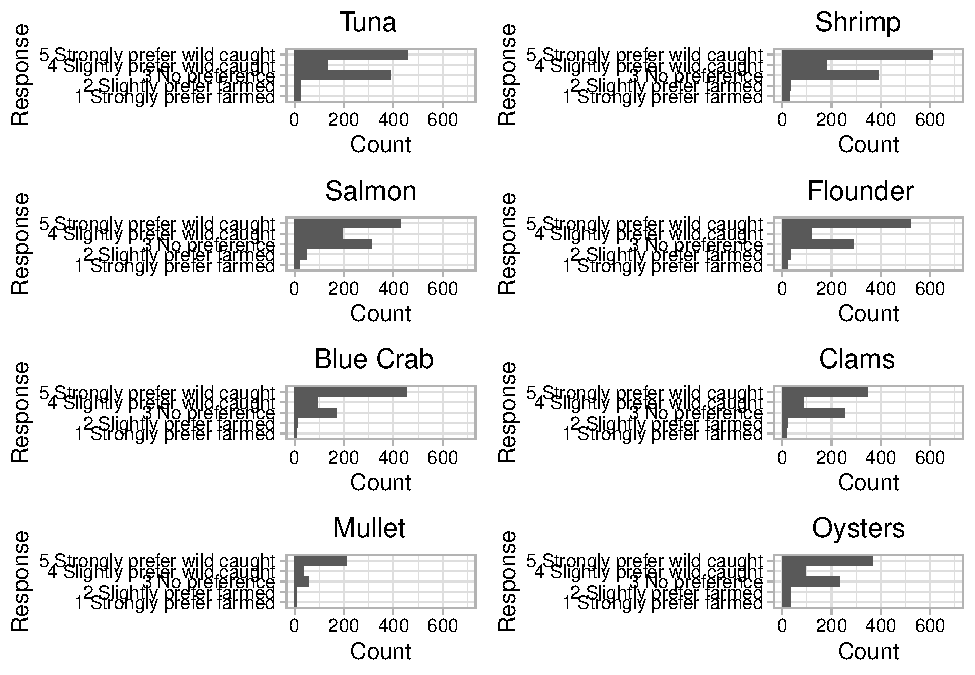
\includegraphics{Final_rmd_files/figure-latex/preference-1.pdf}
\caption{Do you prefer wild-caught or farmed versions of these seafood?}
\end{figure}

On the whole, respondents seem to have some degree of preference for
wild caught seafood or don't have any preference between wild caught and
farmed seafood. However, very few respondents identified any degree of
preference for farmed fish.

Figure 3 does a clear job of showing that the preference trends remain
relatively uniform across all species but with a couple interesting
points. For those species that respondents said they consumed less
often, Mullet and Blue Crab, respondents showed a larger ``stronger
preference for wild caught.'' Meanwhile, for those species that
respondents said they consumed more often, Tuna, Shrimp, and Salmon,
respondents identified ``no preference'' between farmed and wild-caught
a little more readily.

\newpage

\hypertarget{question-2a-what-qualities-do-consumers-associate-with-seafood}{%
\subsection{Question 2a: What qualities do consumers associate with
seafood?}\label{question-2a-what-qualities-do-consumers-associate-with-seafood}}

\begin{figure}
\centering
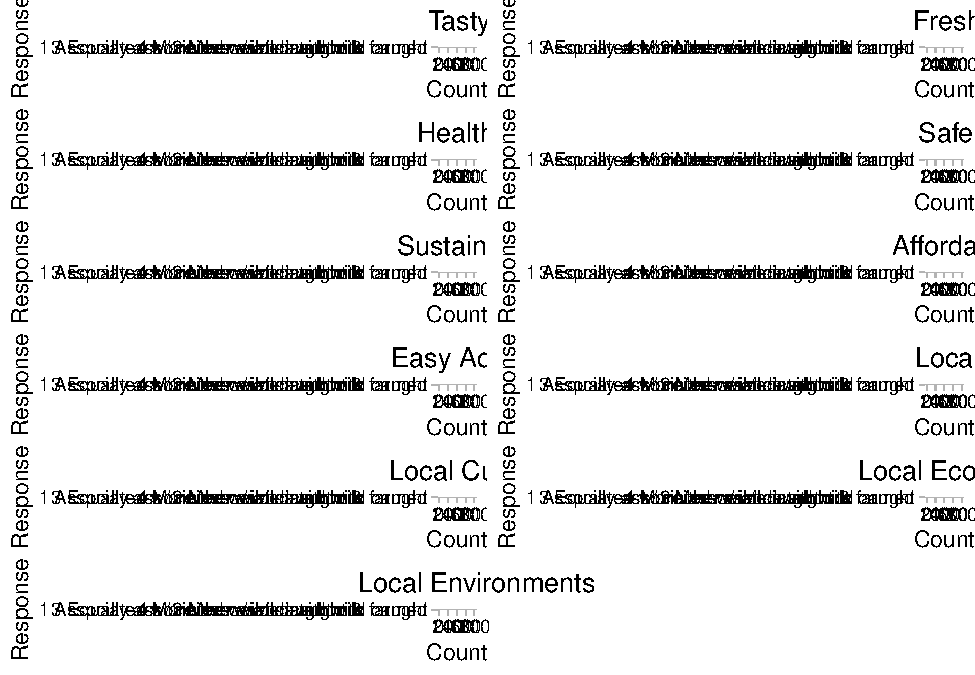
\includegraphics{Final_rmd_files/figure-latex/qualities-1.pdf}
\caption{How do you associate the following qualities with wild
vs.~farmed seafood?}
\end{figure}

There is quite the spread in associations of particular qualities with
farmed or wild-caught seafood, as shown in figure 4. Specifically, it
seems as though respondents tend to associate tasty, fresh, safe,
healthy, and the various local categories more heavily with wild-caught
seafood. However, respondents tent to associate sustainability, easy
access, and affordability more heavily with farmed seafood.

\hypertarget{question-2b-what-qualities-do-consumers-value-in-seafood}{%
\subsection{Question 2b: What qualities do consumers value in
seafood?}\label{question-2b-what-qualities-do-consumers-value-in-seafood}}

\begin{figure}
\centering
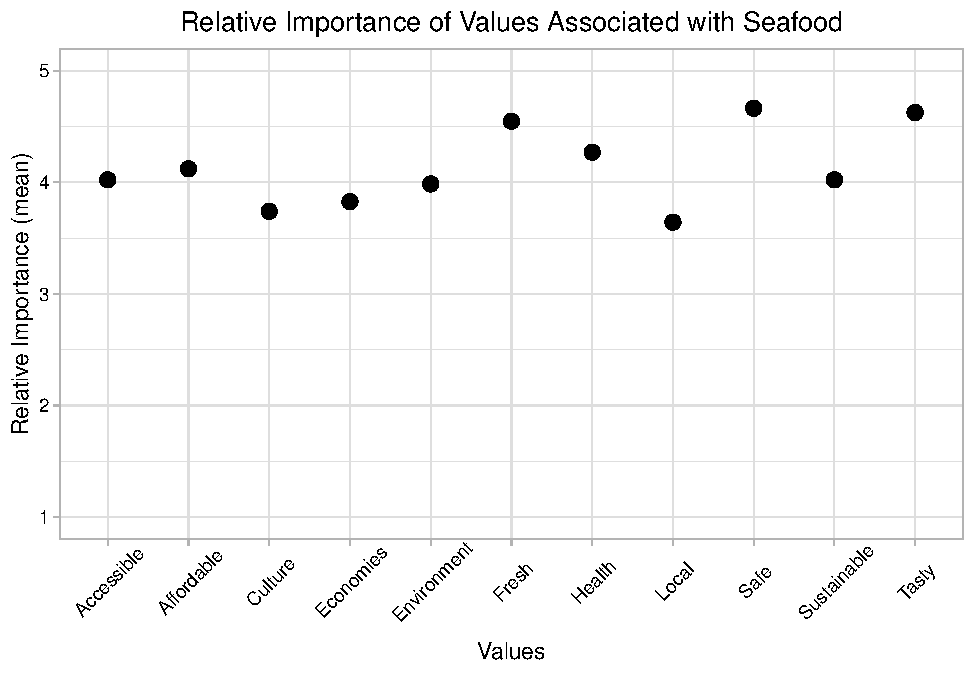
\includegraphics{Final_rmd_files/figure-latex/importance-1.pdf}
\caption{How important are the following qualities?}
\end{figure}

In figure 5, we can see that respondents prioritized certain qualities
like safety, tastiness, freshness, and healthiness of the seafood but
didn't seem to place as much emphasis on other qualities like whether
the seafood was farmed or wild.

\newpage

\hypertarget{question-3-are-valued-seafood-qualities-predicted-by-demographic-variables-such-as-age-or-education-level}{%
\subsection{Question 3: Are valued seafood qualities predicted by
demographic variables such as age or education
level?}\label{question-3-are-valued-seafood-qualities-predicted-by-demographic-variables-such-as-age-or-education-level}}

Age is a predictor of the value respondents placed on the freshness if
their seafood, with folks older than 19 placing more value on the
freshness of their seafood. The low p-value (\textless.05) indicates
that this association is statistically significant. However, the low r
squared value means that age explains only \textasciitilde3.69\% of the
variability in the data. Education is also a predictor of how a
respondent values freshness. The low p-value again indicates that this
association is statistically significant, though the r squared of 2.07\%
means that it doesn't explain much variability in the data. Political
party is not a significant predictor of the value a respondent places on
the freshness of their seafood as told by the high p-value of .4211.

Age is a predictor of the value respondents placed on the local nature
of their seafood. The low p-value (\textless.05) indicates that this
association is statistically significant. However, the low r squared
value means that age explains only \textasciitilde1.78\% of the
variability in the data. Education is also a predictor of how a
respondent values the local nature of their seafood. The low p-value
again indicates that this association is statistically significant,
though the r squared of 1.48\% means that it doesn't explain much
variability in the data. Political party is not a significant predictor
of the value a respondent places on the local nature of their seafood as
told by the high p-value of .2403.

Age is a predictor of the value respondents placed on the taste of their
seafood. The low p-value (\textless.05) indicates that this association
is statistically significant. However, the low r squared value means
that age explains only \textasciitilde1.41\% of the variability in the
data. Education is also a predictor of how a respondent values the taste
of their seafood. The low p-value again indicates that this association
is statistically significant, though the r squared of 0.98\% means that
it doesn't explain much variability in the data. Political party is not
a significant predictor of the value a respondent places on the taste of
their seafood as told by the high p-value of .1333.

Age overall was not a significant predictor of how respondents valued
health (p\textgreater0.05). However, the age ranges of 50-59 and 60-69
were significant and the estimates were positive, indicating that
respondents in these age ranges valued health as a quality of seafood
more than teenagers. Education was a significant predictor of how
respondents valued health (p = 0.007). All estimates were positive,
indicating that a high school education or more predicted that
respondents would value health in their seafood more highly. Political
party was not a significant predictor of how respondents valued health
(p\textgreater0.05).

\newpage

\hypertarget{summary-and-conclusions}{%
\section{Summary and Conclusions}\label{summary-and-conclusions}}

This analysis communicates several key findings--findings that (1)
should inform future inquiries as researchers aim to better understand
community and consumer understandings of seafood and sustainability
issues, and (2) may help researchers make positive strides toward
pursuing education and engagement efforts on these issues.

First, respondents tend to consume certain species of seafood in larger
volumes and at higher frequencies than other species. Shrimp, Tuna, and
Salmon top the list. Meanwhile, respondents do not consume as much
Mullet, Blue Crab, Oyster, or Clams. These consumption practices and
patterns are important because they substantiate broader trends within
fisheries management; certain species are subject to the bulk of
over-fishing concerns because of their marketability to consumers.
Therefore, addressing over-fishing concerns and pursuing education and
engagement efforts may be most effectively targeted at only a handful of
species.

Second, respondents noted some preference for wild-caught seafood across
all species, though many respondents noted that they didn't have a
preference between wild-caught and farmed seafood. The preference for
wild-caught seafood was stronger for species respondents tend to consume
less often, meanwhile a lack of preference was more prevalent for
species respondents consumed more often. These results have bearing on
education efforts surrounding the pros and cons and relative
sustainability of farmed versus wild-caught seafood.

Third, respondents associated different qualities more and less heavily
with farmed and wild-caught seafood. For instance, respondents tend to
think of wild-caught seafood as more associated with tastiness,
freshness, safety, and health. Furthermore, respondents associate
wild-caught seafood with local culture, local economies, etc. Meanwhile,
Respondents identified farmed seafood as having a stronger relationship
with sustainability, easy access, and affordability. The association
respondents have between farmed seafood and sustainability is
particularly interesting and reflects a substantial opportunity for
education \& outreach. Furthermore, respondents prioritize qualities
such as safety, tastiness, freshness, and health but don't prioritize
whether the seafood is framed or wild-caught. Again, these priorities
are worthy of further exploration.

Finally, statistical analysis substantiates this visual inspection of
the data; it indicates that respondents most heavily associate the
qualities of taste, health, and local with wild-caught seafood.
Furthermore, statistical analysis indicates that political party plays a
statistically significant role in determining if a respondent
prioritizes health in seafood selection. Respondents with some level of
college education place a higher value on health.

\newpage

\hypertarget{references}{%
\section{References}\label{references}}

Pauly, D., \& Zeller, D. (2016). Catch reconstructions reveal that
global marine fisheries catches are higher than reported and declining.
Nature Communications,7(1), pp 1-9.

\end{document}
